\newpage 
\chapter{Matlab} 

MATLAB is a language for mathematical computations whose fundamental data types are vectors and matrices. 
\begin{itemize}
    \item Many built-in commands, SVD, FFT and matrix inversion; 
    \item Built for large-scale scientific computing and small- and medium- scale experimentation in NLA.
\end{itemize}

\section{Exp 1: Discrete Legendre Poly} 
The following lines of MATLAB construct this matrix and compute its reduced QR factorization.
\begin{lstlisting}[language=Matlab]
    x = (-128:128)'/128;
    A= [x.^0 x.^1. x.^2 x.^3] ;
    [Q,R] = qr(A,0);
\end{lstlisting}
The columns of the matrix $Q$ are essentially the first four Legendre polynomials. They differ slightly, by amounts close to plotting accuracy. They also differ in normalization, since a Legendre polynomial should satisfy $P_k(1)=1$. We can fix this by diving each column of $Q$ by its final entry. 
\begin{lstlisting}[language=Matlab] 
    scale = Q(257,:);
    Q = Q*diag(1 ./scale);
    plot (Q)
\end{lstlisting}
 
The result of our computation is a plot that looks just like Figure 7.1. 

\section{Exp 2: Classical vs. Modified Gram-Schmidt} 

First, we construct a square matrix $A$ with random singular vbectors and widely varying singular values spaced by factors of $2$ between $2^{-1}$ and $2^{-80}$.  
\begin{lstlisting}[language=matlab]
    [U,X] = qr(randn(80)); &\Comment{ Set $U$ to a random orthogonal matrix. } &
    [V,X] = qr(randn(80)); &\Comment{ Set $V$ to a random orthogonal matrix. } &
    S = diag(2.^(-1:-1:-80));   &\Comment{ Set $S$ to a diagonal matrix with exponentially graded entries. } &
    A= U*S*V; &\Comment{ Set $A$ to a matrix with these entries as singular values. } &
\end{lstlisting}

In the following code, the programs clgs and mgs are MATLAB implementations, not listed here, of Algorithms 7.1 and 8.1.

\begin{lstlisting}[language=Matlab]
   [QC, RC] = clgs(A); &\Comment{ Compute a factorization QR by classical GS} & 
   [QM, RM] = mgs(A); &\Comment{ Compute a factorization QR by modified GS } &
\end{lstlisting}

Finally, we plot the diagonal entries $r_{jj}$.  
%────────────────────────────────────────
\begin{figure}[H]
    \centering
    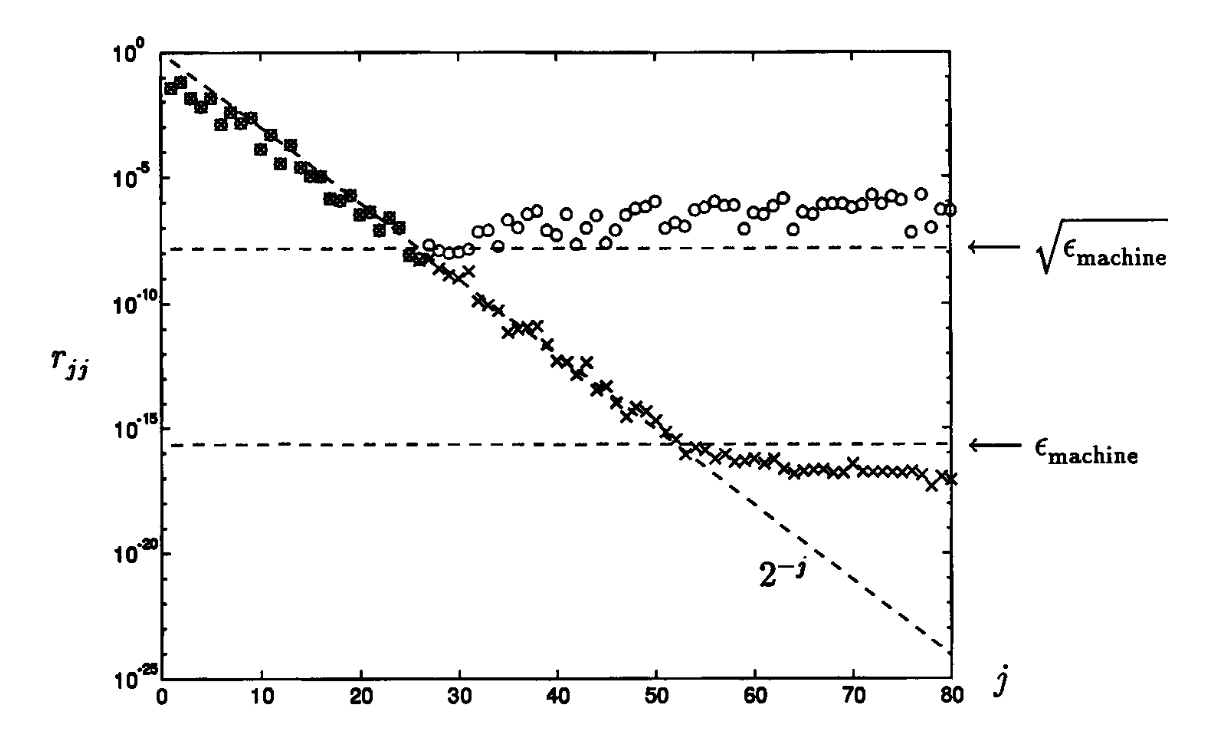
\includegraphics[width=0.8\textwidth]{figures/9-1.png}
    \label{fig 9.1} 
    \caption{The classical GS is represented by circles while the modified GS is represented by crosses.}
\end{figure}
%────────────────────────────────────────
Notice that: 
\begin{itemize}
    \item $r_{jj}$ is close to $2^{-j}$. This is because 
    \begin{align*}
        A=2^{-1} u_1 v_1^*+2^{-2} u_2 v_2^*+2^{-3} u_3 v_3^*+\cdots+2^{-80} u_{80} v_{80}^*, \\ 
        a_j=2^{-1} \bar{v}_{j 1} u_1+2^{-2} \bar{v}_{j 2} u_2+2^{-3} \bar{v}_{j 3} u_3+\cdots+2^{-80} \bar{v}_{j, 80} u_{80} .
    \end{align*}
    Here $v_{ji}$ are almost constants $ \approx 0.1 $. In fact $u_i \approx q_i$ and $r_{ii} \approx 0.1*2^{-i}$.  
    \item For classical GS, $r_{jj}$ stop at $10^{-8}$ while the modified GS is down to the order of $10^{-16}$, which is the level of machine epsilon.   
\end{itemize}
Hence, the modified GS is more stable.  Consequently the classical GS is rarely used, except sometimes on parallel computers in situations where advantages related to communication may outweigh the disadvantage of instability.

\section{Exp 3: Numerical Loss of Orthogonality} 
 In floating point arithmetic, these algorithms may produce vectors $q_j$ that are far from orthogonal. The loss of orthogonality occurs when $A$ is close to rank-deficient, and, like most instabilities, it can appear even in low dimensions.

Starting on paper rather than in MATLAB, consider the case of a matrix
$$
A=\left[\begin{array}{ll}
0.70000 & 0.70711 \\
0.70001 & 0.70711
\end{array}\right]
$$
on a computer that rounds all computed results to five digits of relative accuracy (Lecture 13). The classical and modified algorithms are identical in the $2 \times 2$ case. At step $j=1$, the first column is normalized, yielding
$$
r_{11}=0.98996, \quad q_1=a_1 / r_{11}=\left[\begin{array}{c}
0.70000 / 0.98996 \\
0.70001 / 0.98996
\end{array}\right]=\left[\begin{array}{c}
0.70710 \\
0.70711
\end{array}\right]
$$
in five-digit arithmetic. At step $j=2$, the component of $a_2$ in the direction of $q_1$ is computed and subtracted out:
$$
\begin{aligned}
& r_{12}=q_1^* a_2=0.70710 \times 0.70711+0.70711 \times 0.70711=1.0000 \\
& v_2=a_2-r_{12} q_1=\left[\begin{array}{l}
0.70711 \\
0.70711
\end{array}\right]-\left[\begin{array}{l}
0.70710 \\
0.70711
\end{array}\right]=\left[\begin{array}{l}
0.00001 \\
0.00000
\end{array}\right]
\end{aligned}
$$
again with rounding to five digits. This computed $v_2$ is dominated by errors. The final computed $Q$ is
$$
Q=\left[\begin{array}{ll}
0.70710 & 1.0000 \\
0.70711 & 0.0000
\end{array}\right]
$$
On a computer with sixteen-digit precision, we still lose about five digits of orthogonality if we apply modified Gram-Schmidt to the matrix. Here is the MATLAB evidence. The "eye" function generates the identity of the indicated dimension.
\begin{lstlisting}[language=Matlab]
    A = [.70000 .70711 &\Comment{ Define $A$. } &
    .70001 .70711] ;   
    [Q, R] = qr(A); &\Comment{ Compute factor $Q$ by Householder. } &
    norm(Q'*Q-eye(2)) &\Comment{ Test orthogonality of $Q$. } &
    [Q, R] = mgs(A); &\Comment{ Compute factor $Q$ by modified GS. } &
    norm(Q'*Q - eye(2)) &\Comment{ Test orthogonality of $Q$. } &
\end{lstlisting}
The results are: 
\[
    \text { ans }=2.3515 e-16, \quad \text { ans }=2.3014 e-11. 
\]